\subsection{Customer Choice Dynamics}
We first show that every customer exhibits the following behavior: until (s)he reaches the phase transition point $i_0(t)$, she visits $A$ only due to the exogeneity paramaeter, and after that (s)he always visits merchant $A$ till she receives the reward.
This behavior is cyclic, and repeats after every reward redemption.

\begin{lemma} $V(i)$ is an increasing function in $i$ if the following condition holds:
\begin{equation}
R > \frac{(1-\lambda)v}{1-\beta}
\end{equation}
And further, $V(i)$ can be evaluated as:
\begin{equation}
V(i) = \max\left\{ \frac{\lambda \beta V(i+1)+(1-\lambda)v}{1-(1-\lambda)\beta}, \beta V(i+1) \right\}
\end{equation}
\end{lemma}

\begin{proof}
First we show that $V(i)$ is an increasing function in $i$ by induction. We first show that if the condition above is satisfied, $V(k-1) < V(k) = R$. Suppose not, so $V(i) \geq R$. Then we have:
\begin{align*}
V(k-1) &= \lambda \beta V(k) + (1-\lambda)(v+\beta V(k-1)) \\
&= \frac{\lambda \beta R + (1-\lambda)v}{1-(1-\lambda)\beta} \\
&< \frac{\lambda \beta R + (1-\beta)R}{1-(1-\lambda)\beta} \\
&= \frac{R(1-(1-\lambda)\beta)}{1-(1-\lambda)\beta} = R
\end{align*}
But this is a contradiction, so $V(k-1) < V(k)$. Now assume $V(i+1) < V(i+2)$ for some $i < k-2$, we will show that this implies $V(i) < V(i+1)$. Suppose not, so $V(i) \geq V(i+1)$. As we did before we may upper bound $V(i)$.
\begin{align*}
V(i) &= \lambda \beta V(i+1) + (1-\lambda)(v+\beta V(i)) \\
&\leq (1-\lambda)v + \beta V(i) \\
\iff V(i) &\leq \frac{(1-\lambda)v}{1-\beta}
\end{align*}
But because $V(i+1) < V(i+2)$, we may lower bound $V(i+1)$.
\begin{align*}
V(i+1) &\geq \lambda \beta V(i+2) + (1-\lambda)(v+\beta V(i+1)) \\
&= (1-\lambda)v + (1-\lambda)\beta V(i+1) + \lambda \beta V(i+2) \\
&> (1-\lambda)+\beta V(i+1) \\
\iff V(i+1) &> \frac{(1-\lambda)v}{1-\beta}
\end{align*}
Again, we have a contradiction, so $V(i) < V(i+1)$, and $V(i)$ is an increasing function in $i$. Now we prove the second claim. We have the following:
\begin{align*}
V(i) &= \lambda \beta V(i+1) + (1-\lambda)\max\{v +\beta V(i), \beta V(i+1) \} \\
&= \max\{\lambda \beta V(i+1) + (1-\lambda)(v+\beta V(i)), \beta V(i+1) \}
\end{align*}

Assuming $V(i)$ is the left term in the above maximum, we may solve the equation for that term.
\begin{gather*}
V(i) = \lambda \beta V(i+1) + (1-\lambda)(v+\beta V(i)) \\
(1-(1-\lambda)\beta) V(i) = \lambda \beta V(i+1) + (1-\lambda)v \\
V(i) = \frac{\lambda \beta V(i+1) + (1-\lambda)v}{1-(1-\lambda)\beta}
\end{gather*}
And we get our claim.
\end{proof}

\begin{theorem} Suppose $V(i)$ is an increasing function in $i$ and consider a customer with look-ahead parameter $t$. A phase transition occurs after (s)he makes $i_0(t)$ visits to firm $A$, where $i_0(t)$ is given by:
\begin{equation}
  i_0(t)=\begin{cases}
    k-\Delta \equiv i_0, & \text{if $t \geq \Delta$}.\\
    k-t, & \text{otherwise}.
  \end{cases}
\end{equation}
with 
\begin{align}
\Delta &= \left\lfloor \log_{\beta}\left(\frac{v}{R(1-\beta)}\right)\right\rfloor
\end{align}
\end{theorem}

\begin{proof}
First we solve for the condition on $V(i+1)$ for us to choose firm $A$ over $B$ willingly.
\begin{gather*}
\beta V(i+1) > \frac{\lambda \beta V(i+1) + (1-\lambda)v}{1-(1-\lambda)\beta} \\
\iff \beta V(i+1) \left(1-\frac{\lambda}{1-(1-\lambda)\beta} \right) > \left(\frac{1-\lambda}{1-(1-\lambda)\beta} \right) v \\
\iff \beta V(i+1) \left(\frac{1-(1-\lambda)\beta -\lambda}{1-(1-\lambda)\beta} \right) > \left(\frac{1-\lambda}{1-(1-\lambda)\beta} \right) v \\
\iff \beta V(i+1) \left(\frac{(1-\lambda)(1-\beta)}{1-(1-\lambda)\beta} \right) > \left(\frac{1-\lambda}{1-(1-\lambda)\beta} \right) v \\
\iff \beta V(i+1) > \frac{v}{1-\beta} \\
\iff V(i+1) > \frac{v}{\beta(1-\beta)}
\end{gather*}
Let $i_0$ be the minimum state $i$ such that the above holds, so in particular $V(i_0) \le \frac{v}{\beta(1-\beta)}$ but $V(i_0+1) > \frac{v}{\beta(1-\beta)}$. We know because $V$ is increasing in $i$, this point is indeed a phase transition: $V(i) > \frac{v}{\beta(1-\beta)}$ for all $i > i_0$, so after this point, the customer always chooses firm $A$. We may compute $V(i_0)$ easily using this fact.
\begin{equation*}
V(i_0) = \beta V(i_0+1) = \cdots = \beta^{k-i_0}V(k) = \beta^{k-i_0}R
\end{equation*}
Thus, we have the following:
\begin{gather*}
\beta^{k-i_0} \le \frac{v}{R\beta(1-\beta)} < \beta^{k-(i_0+1)} \\ 
\iff k-i_0 \ge \log_{\beta}\left(\frac{v}{R\beta(1-\beta)} \right) > k-(i_0+1) \\
\iff i_0 \le k - \log_{\beta}\left(\frac{v}{R(1-\beta)} \right) + 1 < i_0 + 1\\
\iff i_0 = k - \left\lfloor \log_{\beta}\left(\frac{v}{R(1-\beta)}\right) \right\rfloor \equiv k-\Delta
\end{gather*}

The above dependence reduces to the following after incorporating the look-ahead distribution:

\begin{equation*}
  i_0(t)=\begin{cases}
    i_0, & \text{wp } p,\\
    k, & \text{wp } 1-p.
  \end{cases}
\end{equation*}
\end{proof}

{\arpit Discussion around what do the $i_0$ dependencies mean.}

{\arpit Discussion around setting $i_0 = 0$}

\subsection{Merchant Objective Dynamics}
We substitute the value of the phase transition point obtained above in the rate of revenue equations to reevaluate them. 
And since we assume that $\lambda$ and $t$ are drawn indepent of each other, we can separate the expectation terms and evaluate them sequentially, first over $t$, then over $\lambda$. This reduces the rate of revenues as follows:

\begin{align*}
RoR_A =& \underset{\lambda, t}E\left[\frac{k-R}{i_0(t)/\lambda + k - i_0(t)}\right]\\
                                       =& \underset{\lambda}E\left[p\cdot\frac{k-R}{i_0/\lambda + k - i_0} + (1-p)\frac{\lambda(k-R)}{k}\right]\\
                                       =& \underset{\lambda}E\left[p\cdot\frac{\lambda(k-R)}{k\lambda + i_0(1-\lambda)} + (1-p)\frac{\lambda(k-R)}{k}\right]\\
                                       =& p\cdot\frac{k-R}{b(k-i_0)^2}\cdot\left(b(k-i_0) - i_0 \log\left(1 + \frac{b(k-i_0)}{i_0}\right)\right) + (1-p)\frac{b(k-R)}{2k}\\
                                       =& p\cdot\frac{k-R}{b\Delta^2}\cdot\left(b\Delta - (k-\Delta)\log\left(1+\frac{b\Delta}{k-\Delta}\right)\right) + (1-p)\frac{b(k-R)}{2k}\\
                                       =& p\cdot\frac{k-R}{\Delta}\cdot\left(1 - \frac{k-\Delta}{b\Delta}\log\left(1+\frac{b\Delta}{k-\Delta}\right)\right) + (1-p)\frac{b(k-R)}{2k}
\end{align*}

\begin{align*}
RoR_B =& \underset{\lambda, t}E\left[\frac{(i_0(t)\lambda - i_0(t))(1-v)}{i_0(t)/\lambda + k - i_0(t)}\right]\\
                                     =& \underset{\lambda}E\left[p\cdot\frac{(i_0/\lambda - i_0)(1-v)}{i_0/\lambda + k - i_0} + (1-p)\frac{(k/\lambda - k)(1-v)}{k/\lambda}\right]\\
                                     =& \underset{\lambda}E\left[p\cdot\frac{i_0(1-\lambda)(1-v)}{k\lambda + i_0(1-\lambda)} + (1-p)(1-\lambda)(1-v)\right]\\
                                     =& p\cdot\frac{i_0(1-v)}{b(k-i_0)^2}\left(k\log\left(1+\frac{b(k-i_0)}{i_0}\right) - b(k-i_0)\right) + (1-p)(1-\frac{b}{2})(1-v)\\
                                     =& p\cdot\frac{(k-\Delta)(1-v)}{b\Delta^2}\left(k\log\left(1+\frac{b\Delta}{k-\Delta}\right) - b\Delta\right) + (1-p)(1-\frac{b}{2})(1-v)\\
                                     =& p\cdot\frac{(k-\Delta)(1-v)}{\Delta}\left(\frac{k}{b\Delta}\log\left(1+\frac{b\Delta}{k-\Delta}\right) - 1\right) + (1-p)(1-\frac{b}{2})(1-v)\\
\end{align*}

\subsubsection{Proportional Promotion Budgeting}
First we look into the case when $A$ sets its reward value $R$ proportional to the product of the distance to the reward $k$ and the discount value $v$ provided by merchant $B$: \ie~ $R = \alpha k v$.
We refer to this case as proportional promotion budgeting.
Note $\alpha$ is a constant here.

\begin{theorem}
Under proportional promotion budgeting, the optimal reward distance that $A$ should set is $k = \frac{e}{\alpha(1-\beta)}$ at all values of $b$ as long as $\beta$ is close to 1.
\end{theorem}
\begin{proof}
Recall the previous expression for $RoR_A$. Maximizing this function is equivalent to maximizing the following:
\begin{align*}
\underset{k}\max\{RoR_A\} \Leftrightarrow & \underset{k} \max\left\{\frac{k}{\Delta}\left(1-\frac{k-\Delta}{b\Delta}\log\left(\frac{k-\Delta(1-b)}{k-\Delta}\right)\right)\right\}
\end{align*}
Now let $\theta = \frac{k}{\Delta}$. Then maximizing the above function is equivalent to maximizing the following function w.r.t. $\theta$. Note that $\theta \geq 1$ because $k \geq \Delta$.
\beq\notag
\underset{k}\max\{RoR_A\} \Leftrightarrow \underset{\theta}\max\{f(\theta)\} \Leftrightarrow \underset{\theta}\max\left\{ \theta \left(1-\frac{\theta-1}{b}\log\left(1 + \frac{b}{\theta-1}\right)\right)\right\} 
\eeq

We will show that $f'(\theta) \leq 0$ for all $\theta$ so maximizing $f$ is equivalent to minimizing $\theta$.

\begin{align*}
f'(\theta) &= \frac{2\theta-1+b}{\theta-1+b} - \frac{2\theta-1}{b} \log \left(1+\frac{b}{\theta-1} \right) \\
&= \frac{2\theta-1}{b}\cdot\left(\left(\frac{2\theta-1+b}{\theta-1+b}\right)\left(\frac{b}{2\theta-1} \right) - \log \left(1+\frac{b}{\theta-1} \right)\right) \\
&= \frac{2\theta-1}{b}\cdot\left(\frac{b}{\theta-1+b}+\frac{b^2}{(2\theta-1)(\theta-1+b)} - \log \left(1+\frac{b}{\theta-1} \right)\right)
\end{align*}

Let $g(b, \theta) = \frac{b}{\theta-1+b}+\frac{b^2}{(2\theta-1)(\theta-1+b)} - \log \left(1+\frac{b}{\theta-1} \right)$. 
In the limit of $b \to 0$, it is easy to see that $f'(\theta) = g(b, \theta) = 0$ for all $\theta$ in the domain. 
We now show that for all $\theta$ in the domain and all $0 < b \leq 1$, $\frac{\partial g(b, \theta)}{\partial b} \leq 0$.

\begin{align*}
\frac{\partial g(b,\theta)}{\partial b} &= \frac{\theta-1}{(\theta-1+b)^2}+\frac{1}{2\theta-1}\cdot \frac{2b(\theta-1+b)-b^2}{(\theta-1+b)^2} -\frac{1}{\theta-1+b} \leq 0 \\
&\iff \theta-1 + \frac{2b(\theta-1+b)-b^2}{2\theta-1} \leq \theta-1+b \\
&\iff \frac{b(2\theta-2+b)}{2\theta-1} \leq b \\
&\iff 2\theta-2+b \leq 2\theta-1 \\
&\iff b \leq 1
\end{align*}

Thus we have shown that for all $\theta$, $g(b,\theta) = 0$ as $b \to 0$ and that for all $\theta$ and $0 < b \leq 1$, $g(b,\theta)$ is decreasing. 
These together mean that for all $\theta$ and $b \in [0,1]$, $g(b,\theta) \leq 0$. 
Which implies that $f'(\theta) \le 0$ for all $\theta$ in the domain.
So to maximize $f$, we need to minimize $\theta$.

Now let's look at the quantity $\theta = \frac{k}{\Delta}$.
\begin{align*}
\frac{k}{\Delta} = \frac{k}{\log_\beta\left(\frac{1}{\alpha k(1-\beta)}\right)} \sim \frac{k(1-\beta)}{\log (\alpha k(1-\beta))} 
\end{align*}
The above approximation relies on $\beta$ close to 1. Now this value is minimized at $k = \frac{e}{\alpha(1-\beta)}$. Therefore, for all $b$, the optimal value for $k$ is given by $\frac{e}{\alpha(1-\beta)}$, the value for which $\frac{k}{\Delta}$ is minimized and takes the value $\frac{e}{\alpha}$. 

\end{proof}

{\nolan Discussion about why this theorem makes sense - restriction on $\beta$ is realistic anyway and minimizing $\Delta$ makes sense as well. Also, should we put this proof in the appendix and just give outline in paper?}

The above proof is very intuitive. To maximize revenue, $A$ should minimize $\frac{k}{\Delta}$, which represents the number of visits required for a ``forward-looking'' customer to adopt the reward program. The condition that $\beta$ be close to 1 is not very restrictive, as we expect it to be near 1 in most cases {\nolan (maybe get a citation for this)}. Note that because $k \geq \Delta$, the above also shows $\alpha \leq e$. Finally, observe that under equal-budgeting, we need $k > \frac{1-\lambda}{1-\beta}$ for $V$ to be increasing. We meet this condition when $k = \frac{e}{\alpha(1-\beta)} \geq \frac{1}{1-\beta} \geq \frac{1-\lambda}{1-\beta}$ . 

{\nolan Got rid of figure we had before with dependency on $\beta$ - should we do something to replace it?}

Now we consider the expected revenues of each firm under these conditions.

\beq
\underset{\lambda, t}E[RoR_A] = pk(1-v)\frac{1}{b}\int_0^b \frac{\lambda}{k-(1-\lambda)\Delta} \mbox{ } d\lambda + (1-p)(1-v)\frac{b}{2}
\eeq

\beq
\underset{\lambda, t}E[RoR_B] = pk(1-v)\frac{1}{b}\int_0^b \frac{1-\lambda}{k-(1-\lambda)\Delta} \mbox{ } d\lambda + (1-p)(1-v)\left(1-\frac{b}{2}\right)
\eeq

First notice that the ratio of expected revenues is independent of $v$, the price difference of the two firms. We observe this behavior in our simulations as well. Figure~\ref{fig:eq_budg_vary_v} shows the revenue rates of $A$ and $B$ as a function of $b$ for different values of $v$. We see that the relative rates do not vary with $v$; changing $v$ only changes the absolute revenue rates of each firm, putting more money into the rewards given out. We see that $b$ must be pretty large for firm $A$ to make more money than firm $B$. 

{\nolan Not sure what best figures are now, we can discuss this.}

\begin{figure}[h!]
\begin{centering}
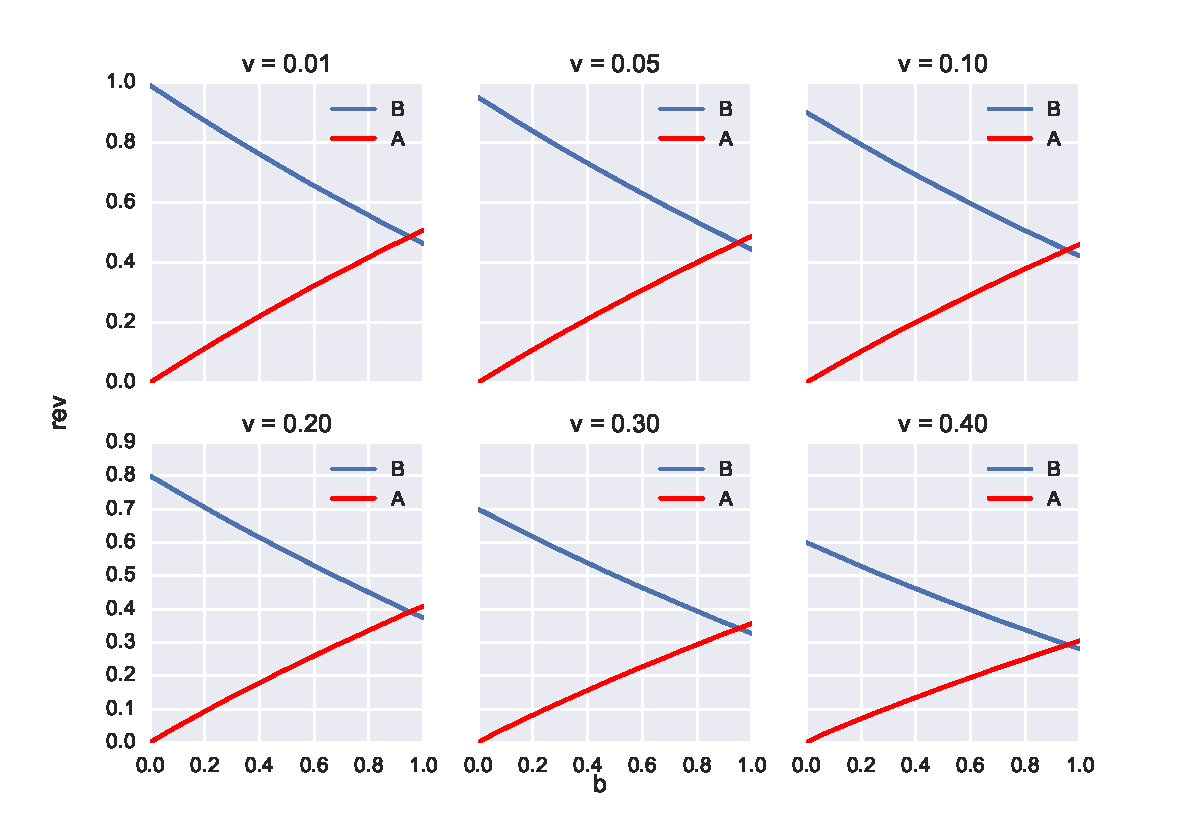
\includegraphics[scale = 0.75]{./figures/eq_budg_vary_v_p05.pdf}
\caption{Rates of revenue for $A$ and $B$ with equal-budgeting as a function of $b$ for various $v$. Fixed $p = 0.5$, $\beta = 0.9$ and $k = e/(1-\beta)$.}
\label{fig:eq_budg_vary_v}
\end{centering}
\end{figure}

[Not sure if we should include] We may solve for the $b$ such that the expected revenues are equal, which occurs if when the following holds (excluding work for now).
\begin{equation*}
b-\frac{2k(k-\Delta)p}{(1-p)b\Delta^2}\log \left(\frac{k-(1-b)\Delta}{k-\Delta} \right) = 1-\frac{p}{1-p} \frac{2k-\Delta}{\Delta}
\end{equation*}

Note from the above that $p$, the probability of a consumer being ``forward-looking'' does affect the ratio of expected rates of revenue. Figure~\ref{fig:eq_budg_vary_p} shows simulation results for the rates of revenue of $A$ and $B$ for various values of $p$ with everything else fixed. We see that as $p$ increases, the $b$ required for the reward program to become more profitable than not using one decreases.

\begin{figure}[h!]
\begin{centering}
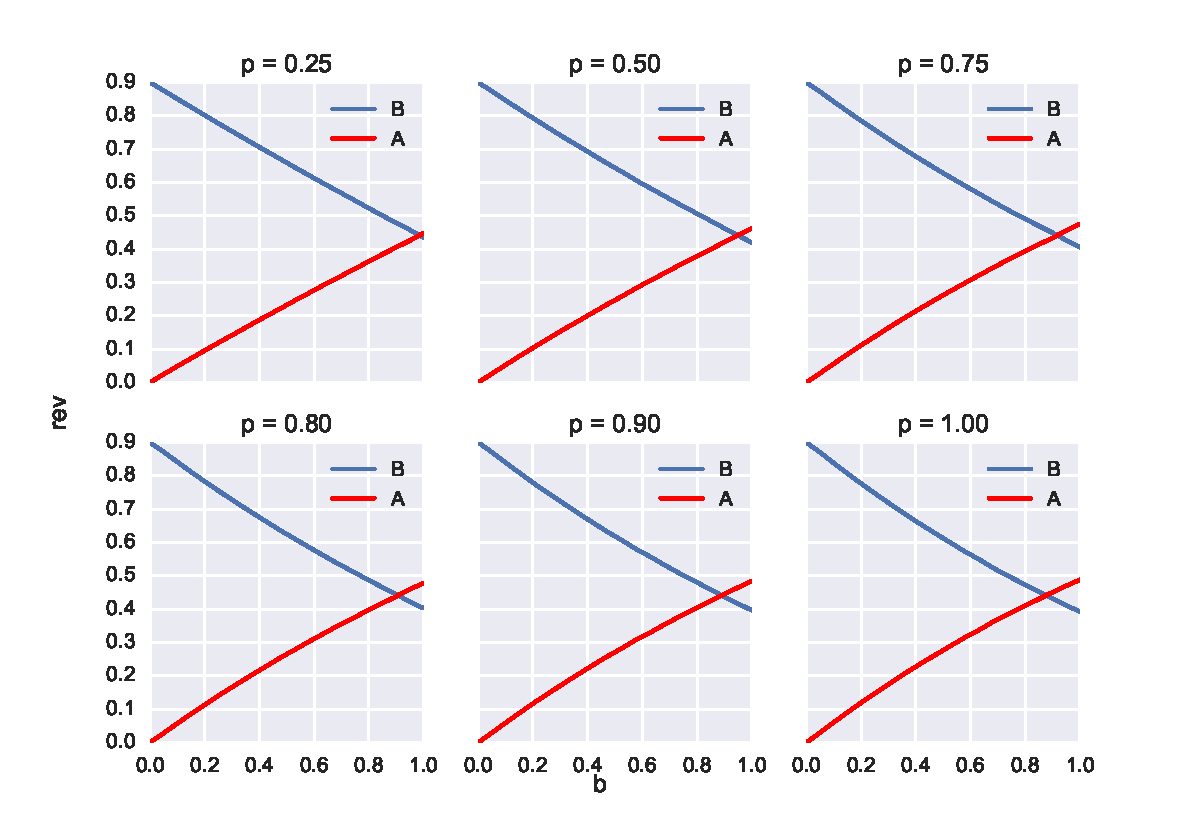
\includegraphics[scale = 0.75]{./figures/eq_budg_vary_p_v01.pdf}
\caption{Rates of revenue for $A$ and $B$ with equal-budgeting as a function of $b$ for various $p$. Fixed $v = 0.1$, $\beta = 0.9$ and $k = e/(1-\beta)$.}
\label{fig:eq_budg_vary_p}
\end{centering}
\end{figure}

{\arpit
\begin{theorem}
When is $RoR_A > RoR_B$ at $i_0 = 0$?
\end{theorem}
}

\begin{figure*}[t!]
\centering
\begin{subfigure}[t]{0.5\textwidth}
\centering
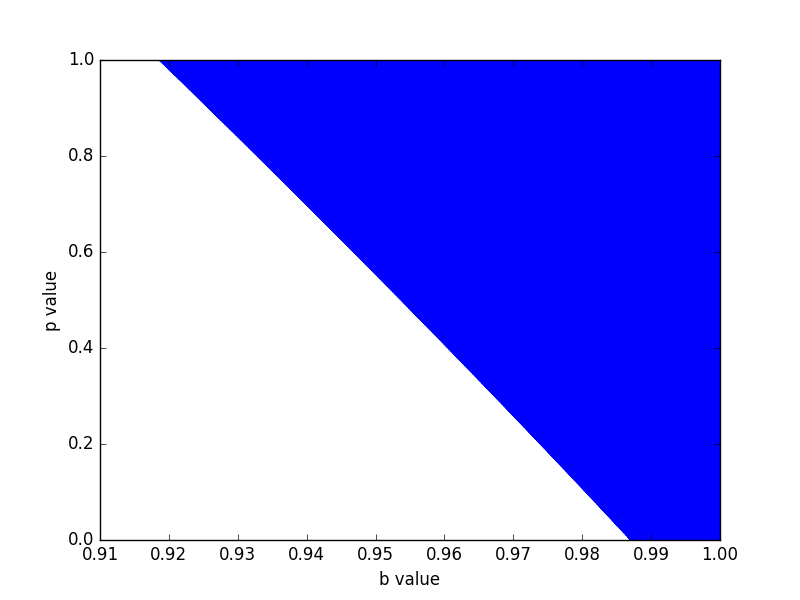
\includegraphics[height=2in]{./figures/bp_pair_rorAB_al0p5_dense.png}
\caption{$\alpha = 0.5$}
\end{subfigure}%
~ 
\begin{subfigure}[t]{0.5\textwidth}
\centering
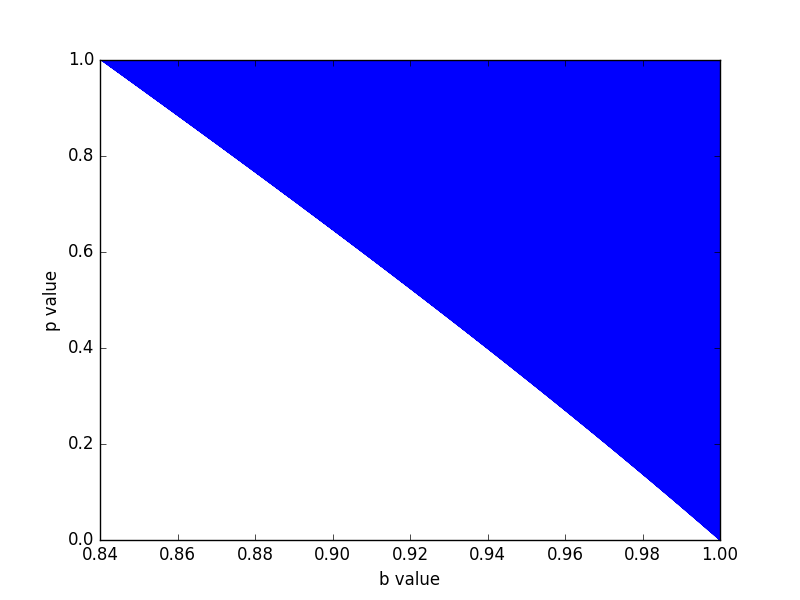
\includegraphics[height=2in]{./figures/bp_pair_rorAB_al1p0_dense.png}
\caption{$\alpha = 1$}
\end{subfigure}
\centering
\begin{subfigure}[t]{0.5\textwidth}
\centering
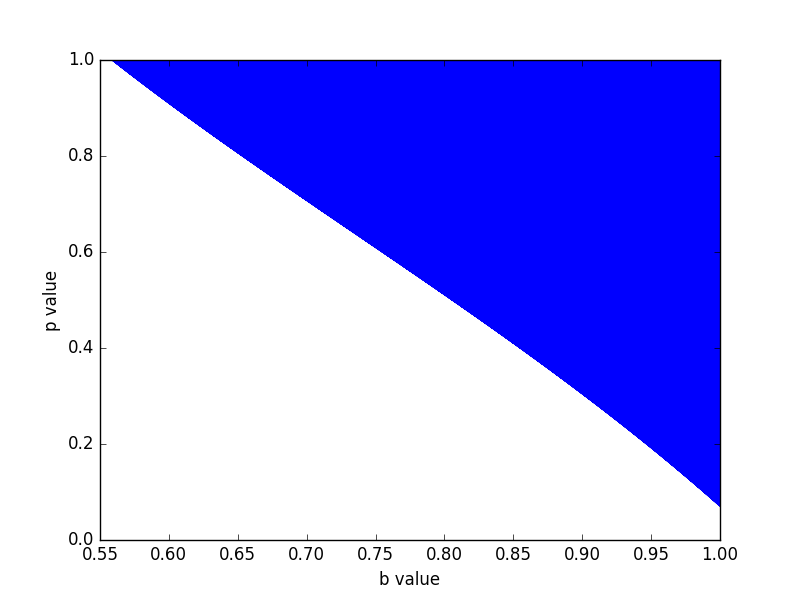
\includegraphics[height=2in]{./figures/bp_pair_rorAB_al2p0_dense.png}
\caption{$\alpha = 2$}
\end{subfigure}%
~ 
\begin{subfigure}[t]{0.5\textwidth}
\centering
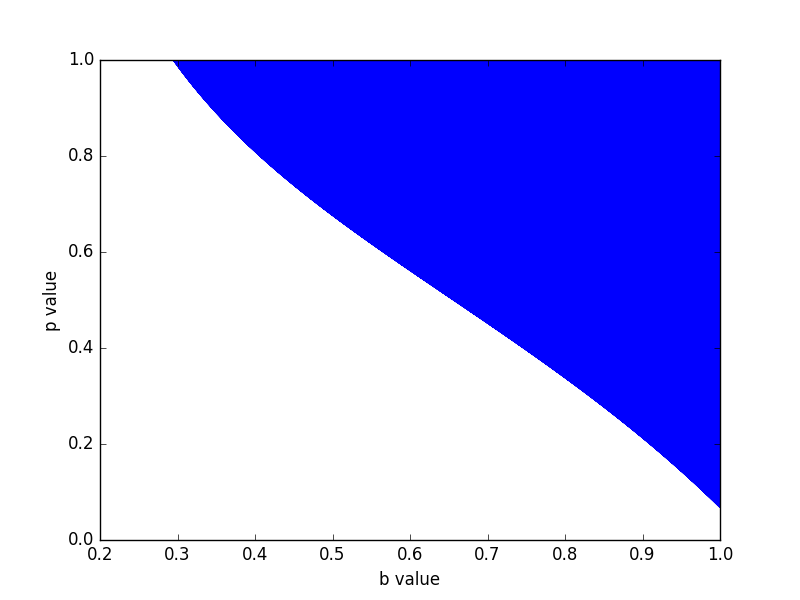
\includegraphics[height=2in]{./figures/bp_pair_rorAB_al2p5_dense.png}
\caption{$\alpha = 2.5$}
\end{subfigure}

\caption{Achievable region of $(b,p)$ pairs where rate of revenue is higher for merchant $A$ for different values of budget proportions $\alpha$. This achievable region is maximized at $\alpha$ close to $e$.}
\end{figure*}


At small values of $b$ the above evaluate to:
\begin{align*}
RoR_A =& p\cdot(k-R)\cdot\frac{b^2}{2i_0} + (1-p)\frac{b^2(k-R)}{2k}\\
                                       =& \frac{b^2(k-R)}{2}\left(\frac{p}{i_0} + \frac{1-p}{k}\right)
\end{align*}

\begin{align*}
RoR_B =& p\cdot\frac{i_0(1-v)}{(k-i_0)^2}\left(bk\frac{(k-i_0)^2}{i_0}- k\frac{b^2(k-i_0)^2}{2i_0^2} \right) + (1-p)(b-\frac{b^2}{2})(1-v)\\
                                     =& p\cdot(1-v)\left(bk- k\frac{b^2}{2i_0}\right) + (1-p)(b-\frac{b^2}{2})(1-v)\\
                                     =& b(1-v)\cdot \left(pk(1-\frac{b}{2i_0}) + (1-p)(1-\frac{b}{2})\right)
\end{align*}

{\arpit Talk about the framework in depth. That this can be used to find optimal $R$ and $k$. Also different distributions can be tested once the framework is ready}


\subsubsection{Non Strategic Merchant $B$, and Unequal Promotion Budgeting}

Now we consider scenarios in which firms $A$ and $B$ have different budgets. First we consider the case where the budgets are still proportional, i.e. $R = \alpha \cdot kv$ for some fixed $\alpha$. Now the expected rate of revenue of $A$ is given by the following, while that of firm $B$ is unchanged. Therefore the ratio of expected revenue rates may now depend on $v$.
\beq
\underset{\lambda, t}E[RoR_A] = pk(1-\alpha v)\frac{1}{b}\int_0^b \frac{\lambda}{k-(1-\lambda)\Delta} \mbox{ } d\lambda + (1-p)(1-\alpha v)\frac{b}{2}
\eeq

Following the same logic of Theorem 3.2, the expected revenue rate of $A$ is maximized at $k = \frac{e}{\alpha(1-\beta)}$ at small values of $b$ (need to do again for larger values). For this value of $k$, $\Delta$ is fixed for all $\alpha$ ($\Delta = \left \lfloor \log_{\beta} \left(\frac{1}{e} \right) \right \rfloor$), so we must have $\alpha \leq \frac{e}{\Delta(1-\beta)}$ for $k \geq \Delta$ to hold. When $\beta = 0.9$, this upperbound on $\alpha$ is about 3.

{\nolan Should proof of this theorem be in the appendix?}

\begin{theorem}
Suppose firm $A$ fixes its price at 1, and firm $B$ chooses a price of $1-v$. Given a consumer distribution defined by $p$ - with probability $p$, a consumer is fully forward looking and probability $1-p$ the customer does not look ahead at all - $b$ - each consumer's monopoly factor to firm $A$ is drawn as $\lambda~\sim Unif(0,b)$ and $\beta$ - the customer's discout factor. Then firm $A$ may choose to give a reward of $\alpha v < 1$ to customers after $k$ visits. It should run a reward program if the following condition holds.
\begin{equation}
\frac{1}{b}\left(1-\frac{e-1}{b}\log \left(1+\frac{b}{e-1} \right) \right) \geq \frac{1-(1-p)(1-\alpha v)}{2pe(1-\alpha v)}
\end{equation}
Define the function on the left-hand side above as $g(b)$.
\end{theorem}

\begin{proof}
Firm $A$ always sells the good for price 1. If it chooses to run a reward program its expected rate of revenue is given by:
\begin{equation*}
\underset{\lambda, t}E[RoR_A] = pk(1-\alpha v)\frac{1}{b}\int_0^b \frac{\lambda}{k-(1-\lambda)\Delta} \mbox{ } d\lambda + (1-p)(1-\alpha v)\frac{b}{2}
\end{equation*}
If it does not run a reward program, then the only visits it will receive are exogenous visits. In this case, its expected rate of revenue is simply $\frac{b}{2}$. We consider a reward program to be profitable if its expected rate of revenue is at least that of the non-reward program expected revenue rate.
\begin{gather*}
pk(1-\alpha v)\frac{1}{b}\int_0^b \frac{\lambda}{k-(1-\lambda)\Delta} \mbox{ } d\lambda + (1-p)(1-\alpha v)\frac{b}{2} \geq \frac{b}{2} \\
\iff \frac{pk(1-\alpha v)}{\Delta}\left(1-\frac{k-\Delta}{b\Delta}\log \left(\frac{k-(1-b)\Delta}{k-\Delta} \right) \right) \geq \frac{b}{2}(1-(1-p)(1-\alpha v)) \\
\iff pe(1-\alpha v)\left(1-\frac{e-1}{b}\log \left(1+\frac{b}{e-1} \right) \right) \geq \frac{b}{2}(1-(1-p)(1-\alpha v)) \\
\iff \frac{1}{b}\left(1-\frac{e-1}{b}\log \left(1+\frac{b}{e-1} \right) \right) \geq \frac{1-(1-p)(1-\alpha v)}{2pe(1-\alpha v)}
\end{gather*}
Where we have used the work from Theorem 3.2 as well as the fact that the optimal $k$ is given by $\frac{e}{\alpha(1-\beta)}$, making $\Delta \approx \frac{1}{1-\beta}$. 
\end{proof}

Note that the above condition on $b$ is rather complicated, so we have plotted it as a function of $b$ below. First we notice that $g(b)$ is decreasing in $b$. So for a fixed evaluation of $x \equiv \frac{1-(1-p)(1-\alpha v)}{2pe(1-\alpha v)}$, we are in one of the following cases:
\begin{enumerate}
\item
$x \geq g(0)$. So no value of $b$ makes the reward program profitable.
\item
$x \leq g(1)$. So any value of $b$ makes the reward program profitable.
\item
$x = g(b_0)$ for some $b_0 \in (0,1)$. So the reward program is profitable for all $b \leq b_0$ and not otherwise.
\end{enumerate}

\begin{figure}[h!]
\begin{centering}
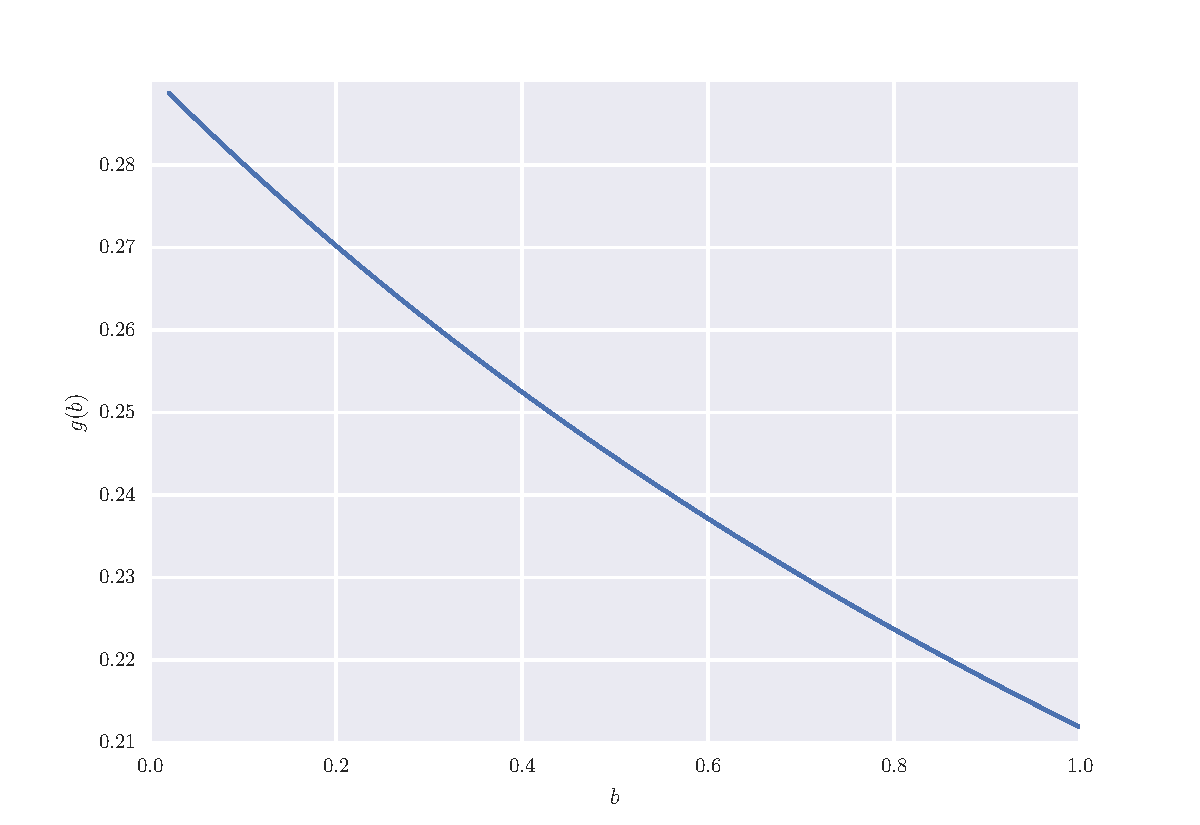
\includegraphics[scale = 0.75]{./figures/b_plot.pdf}
\caption{Function governing profitability of reward program for firm $A$ as a function of $b$.}
\label{fig:b_plot}
\end{centering}
\end{figure}

Now we can take a look at the right hand side of the profitability condition. Let $h(p, \alpha, v) = \frac{1-(1-p)(1-\alpha v)}{2pe(1-\alpha v)}$. It is easy to see that for all values of $p$, $\alpha$ and $v$, $\frac{\partial h}{\partial p} < 0$, $\frac{\partial h}{\partial v} > 0$ and $\frac{\partial h}{\partial \alpha} > 0$. These partial derivative signs mean that as $p$ increases (fixing $v$ and $\alpha$), the interval of profitable $b$'s can only increase. This result make sense intuitively - as the $p$ increases, the number of consumers looking ahead does as well, so more people adopt the reward program. However, increasing either $\alpha$ or $v$ (keeping others fixed), the interval of profitable $b$'s can only decrease. Thus, increasing the reward while keeping $p$ fixed means that in order for the reward program to remain profitable, the profits earned without the reward program must simultaneously decrease, which occurs with decreasing $b$.
